\section{Methods}
\label{sec:methods}

\tab \textbf{Experimental design and data processing.} The laboratory has access to two experimental rooms that enable state-of-the-art experimentation on the retina. From my point of view, it is a golden ticket to original and good quality data. I am learning how to retrieve multi-electrode array experimental data, including semi-automatized spike sorting and cell typing. This process can take up to an entire day for a single experiment. I am also able to share my programming skill to help and improve the data pipeline of the laboratory. This part of my project includes design of experimental stimulus, trustworthy sanity checks and high quality data visualization. %Comment: Same remark for this paragraph.

%Method section ? 
To study fast adaptation, we use a simple stimulus consisting of an adaptation frame (either gray or a checkerboard or its inversion) followed in 400ms by one of three handpicked natural images. Each pair is repeated 1000 times. But each time, the natural images are slightly perturbed using a random checkerboard pattern. This enables the computation of the selectivity of the cell specifically on a local point of a stimulus space containing the natural image of interest (Figure \ref{fig:LSTA}). We refer to it as LSTA \citep{goldin_context-dependent_2022}. One of the challenge here is to be able to identify cells that show fast adaptation in response to our manually designed visual stimulus. For such cells, the LSTA would be different depending on the adaptation that preceded the natural image. %Not sure about the last 3 sentences. The point of this is to see if LSTA is changed by 

\begin{figure}
    \centering
    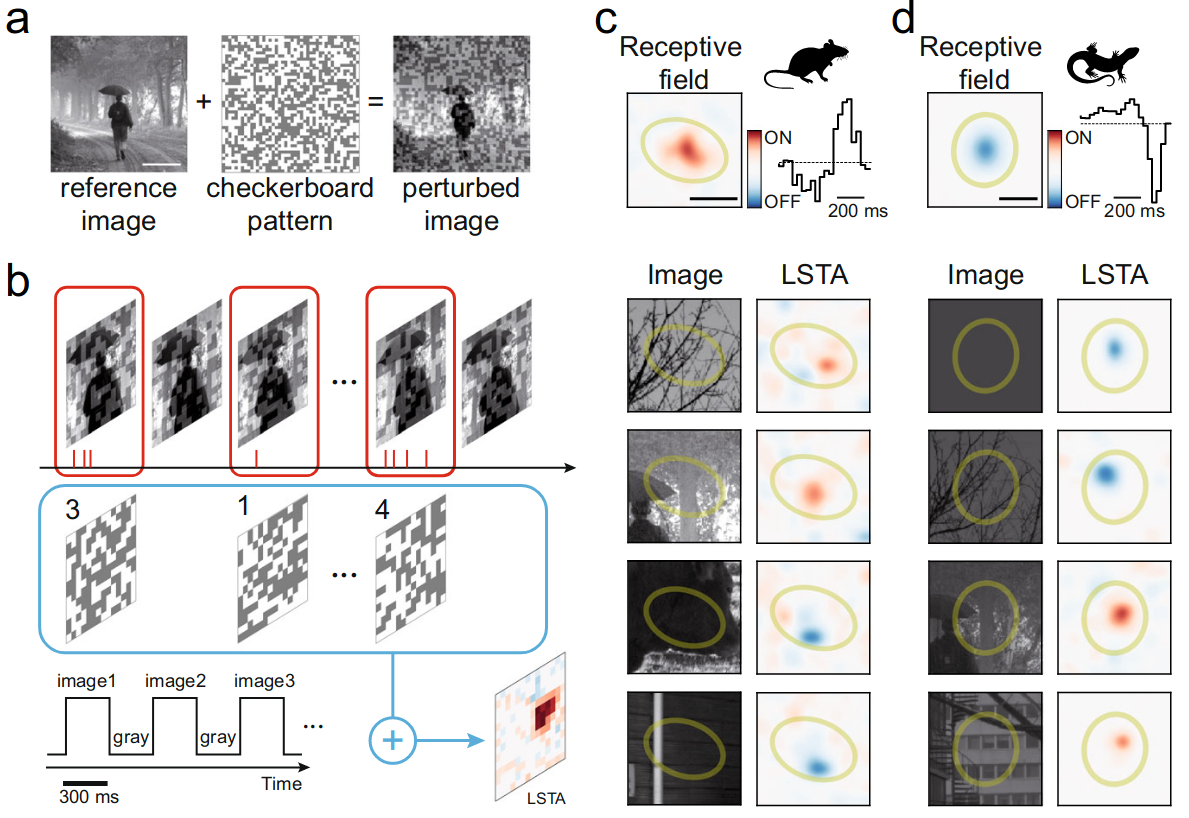
\includegraphics[width=\textwidth]{images/LSTAExplain.png}
    \caption{\textbf{Computation of local sensitivity.} Figure from \citep{goldin_context-dependent_2022} \textbf{a}. Natural images are perturbed with checkerboards. Scale bar = 500 $\mu m$. \textbf{b}. A random sequence of perturbed natural images is being flashed. A gray frame separates all flashes. To compute LSTA, we average all different perturbations weighed by the number of spikes they evoked. \textbf{c} An example of LSTA for a cell of the retina of a mouse. On top, the spatial and temporal receptive field of the cell, as classically used. On the bottom, the LSTA of the cell (right) for different natural images (left).  A green ellipse fitted on the classical spatial field is shown on the LSTA for reference. \textbf{d} Same than c for an axolotl. Note that the stimulus shown here is slightly different from the one we use to trigger fast adaptation. }
    \label{fig:LSTA}
\end{figure}

\hfill \break

\textbf{Modeling.} This should be the main part of my internship and also the most challenging. We are designing a dynamical model of the retinal fast adaptation. In fact, we mostly look at the evolution of the response from an image to another, meaning that the dynamic we observe only spans two points in time. This reduction makes the model more realistic to study. Most of this job can be summarized as model design, python programming, sensitivity analysis and data fitting. By comparing how different modeling strategies reproduce the observed LSTA in the data, we can gain insight on how fast adaptation to natural scene is implemented in the retina.
%I think what is missing here is what question you want to answer with this. We should discuss this more. 

Our baseline model is the LNLN model of ganglion cell widely used in the literature. Each neuron is encoded as a spatial linear filter chained with a non-linearity (usually an activation linearity in the like of ReLU). A single layer of subunit neurons, representing bipolar cells, converge into a single modeled ganglion cell.  We would like to add temporal dynamics to this model, either by adding a time dimension to the spatial liner filter of the cells or by considering a gain control mechanism. This last mechanism consists in scaling up or down the present output depending on past outputs (Figure \ref{fig:LNLN}) \citep{chen_alert_2013}. 

\begin{figure}
    \centering
    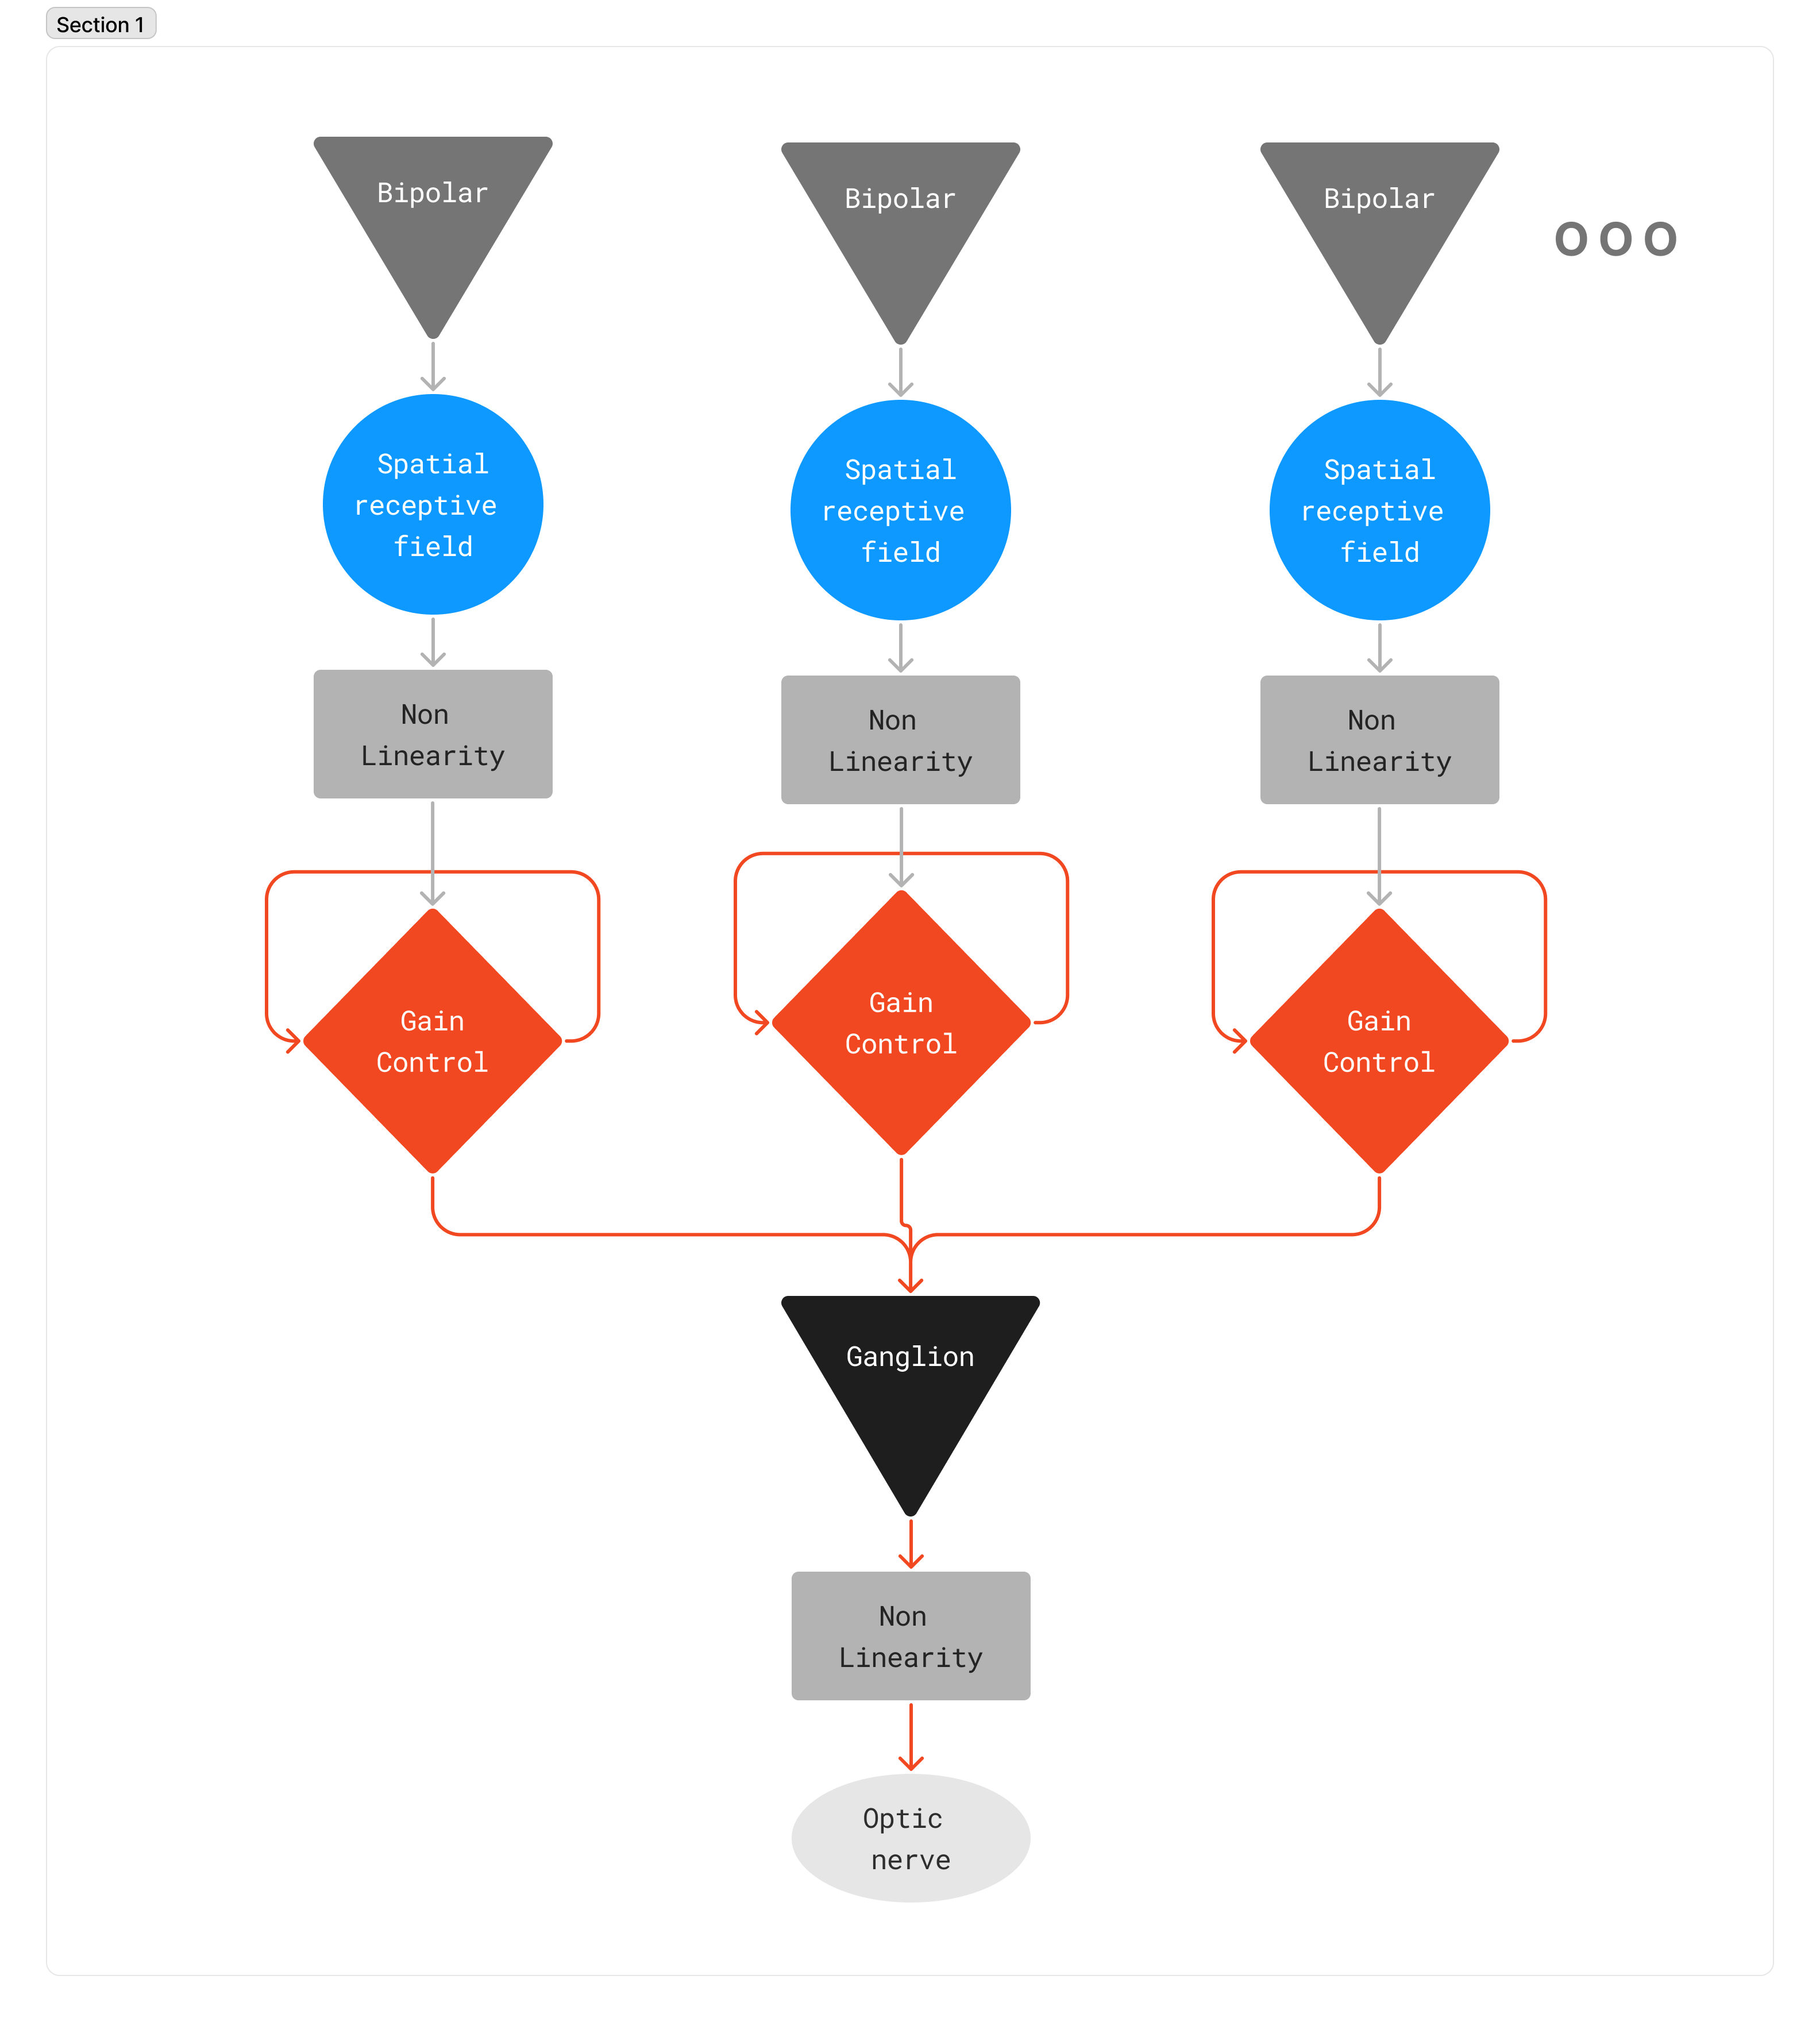
\includegraphics[scale = 0.3]{images/GCModelDiagram.png}
    \caption{\textbf{Quick sketch of a gain control LNLN model.} Each bipolar cell is composed of a linear spatial filter that selectively respond to a part of the scene, a non-linear activation function, and a gain control mechanism that scale its output depending on past events. They all converge into on bipolar cell (forming its own receptive field) of which output is also modeled using a non-linear function.}
    \label{fig:LNLN}
\end{figure}
We will first study our models in a data agnostic manner and study its behavior for different set of parameters. We will then fit it on our own experimental data using an efficient optimization framework in python using strategies developed in the field of machine learning.

\hfill \break

\textbf{Learning about the field.} %Comment: Background knowledge seems redundant with introduction. In practice you should probably separate the introduction of the scientific question etc, and the conditions of your internship. 
Finally, One of my main goal is to learn about the retina and its modeling. To that end, I am doing an extensive study of the literature to build my own library and also get to know the main theories and actors of the field. Through my internship, I also attend the lab weekly science meeting, the lab theoretical journal club as well as some exterior talks in Paris and its area. Finally, I will be attending the main yearly research congress about the retina around the end of my internship. It is called ERM and will be hosted in Tübingen, Germany.
